%!TEX TS-program = xelatex
%!TEX encoding = UTF-8 Unicode
% Awesome CV LaTeX Template for CV/Resume
%
% This template has been downloaded from:
% https://github.com/posquit0/Awesome-CV
%
% Author:
% Claud D. Park <posquit0.bj@gmail.com>
% http://www.posquit0.com
%
%
% Adapted to be an Rmarkdown template by Mitchell O'Hara-Wild
% 23 November 2018
%
% Template license:
% CC BY-SA 4.0 (https://creativecommons.org/licenses/by-sa/4.0/)
%
%-------------------------------------------------------------------------------
% CONFIGURATIONS
%-------------------------------------------------------------------------------
% A4 paper size by default, use 'letterpaper' for US letter
\documentclass[11pt,a4paper,]{awesome-cv}

% Configure page margins with geometry
\usepackage{geometry}
\geometry{left=1.4cm, top=.8cm, right=1.4cm, bottom=1.8cm, footskip=.5cm}


% Specify the location of the included fonts
\fontdir[fonts/]

% Color for highlights
% Awesome Colors: awesome-emerald, awesome-skyblue, awesome-red, awesome-pink, awesome-orange
%                 awesome-nephritis, awesome-concrete, awesome-darknight

\definecolor{awesome}{HTML}{207373}

% Colors for text
% Uncomment if you would like to specify your own color
% \definecolor{darktext}{HTML}{414141}
% \definecolor{text}{HTML}{333333}
% \definecolor{graytext}{HTML}{5D5D5D}
% \definecolor{lighttext}{HTML}{999999}

% Set false if you don't want to highlight section with awesome color
\setbool{acvSectionColorHighlight}{true}

% If you would like to change the social information separator from a pipe (|) to something else
\renewcommand{\acvHeaderSocialSep}{\quad\textbar\quad}

\def\endfirstpage{\newpage}

%-------------------------------------------------------------------------------
%	PERSONAL INFORMATION
%	Comment any of the lines below if they are not required
%-------------------------------------------------------------------------------
% Available options: circle|rectangle,edge/noedge,left/right

\photo{../images/JDL.jpg}
\name{Juan David}{Leongómez}

\position{Profesor Asociado}
\address{Facultad de Psicología, Universidad El Bosque}

\mobile{(+57) 601-6489000 Ext. 1901}
\email{\href{mailto:jleongomez@unbosque.edu.co}{\nolinkurl{jleongomez@unbosque.edu.co}}}
\homepage{jdleongomez.info/es}
\orcid{0000-0002-0092-6298}

% \gitlab{gitlab-id}
% \stackoverflow{SO-id}{SO-name}
% \skype{skype-id}
% \reddit{reddit-id}

\quote{Soy un investigador interesado principalmente en el
comportamiento humano, así como en los métodos cuantitativos y la
ciencia reproducible.}

\usepackage{booktabs}

\providecommand{\tightlist}{%
	\setlength{\itemsep}{0pt}\setlength{\parskip}{0pt}}

%------------------------------------------------------------------------------



% Pandoc CSL macros

\begin{document}

% Print the header with above personal informations
% Give optional argument to change alignment(C: center, L: left, R: right)
\makecvheader

% Print the footer with 3 arguments(<left>, <center>, <right>)
% Leave any of these blank if they are not needed
% 2019-02-14 Chris Umphlett - add flexibility to the document name in footer, rather than have it be static Curriculum Vitae
\makecvfooter
  {06 de febrero de 2024}
    {Juan David Leongómez~~~·~~~Hoja de Vida Resumida}
  {\thepage}


%-------------------------------------------------------------------------------
%	CV/RESUME CONTENT
%	Each section is imported separately, open each file in turn to modify content
%------------------------------------------------------------------------------



\hypertarget{acerca-de-muxed}{%
\section{Acerca de mí}\label{acerca-de-muxed}}

\begin{minipage}[c]{0.9\linewidth}
Soy Profesor Asociado e investigador de \href{https://jdleongomez.info/es/team/}{\textit{\textbf{EvoCo}: Laboratorio de Evolución y Comportamiento Humano}}, y lider del grupo de investigación \href{https://investigaciones.unbosque.edu.co/codec}{\textit{\textbf{CODEC}: Ciencias Cognitivas y del Comportamiento}} (clasificación  \href{https://scienti.minciencias.gov.co/gruplac/jsp/visualiza/visualizagr.jsp?nro=00000000001446}{\textbf{A1}}),  \href{https://www.uelbosque.edu.co/psicologia}{Facultad de Psicología}, \href{https://www.uelbosque.edu.co/}{Universidad El Bosque} en Bogotá, Colombia. Mis intereses de investigación se centran principalmente en la elección de pareja, la comunicación vocal humana y la musicalidad, así como en la bioacústica, la psicoacústica y los efectos hormonales en el comportamiento humano. Me apasionan los métodos cuantitativos y la programación en \textbf{R}, como herramienta para promover la reproducibilidad y la ciencia abierta.
\end{minipage} \begin{minipage}[c]{0.1\linewidth}
\begin{flushright} 
\hfill \href{https://jdleongomez.info/es/team/}{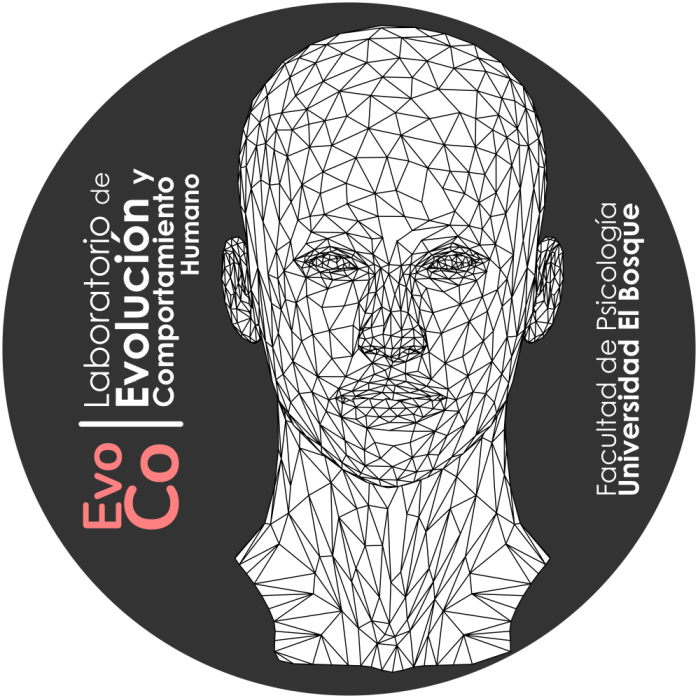
\includegraphics[width=1.5cm, height=1.5cm]{Logo_EvoCo.png}} \newline \href{https://investigaciones.unbosque.edu.co/codec}{
\includegraphics[width=1.5cm, height=1.5cm]{Logo_CODEC.png}}
\end{flushright}
\end{minipage}

\hypertarget{habilidades}{%
\section{Habilidades}\label{habilidades}}

\begin{cvskills}
  \cvskill
    {Programación}
    {\href{https://www.r-project.org/}{\textbf{R}} (avanzado: todo el procesamiento de datos, análisis, diagramas y tablas —e incluso esta HV— hechos en R)}

  \cvskill
    {Informes reproducibles}
    {Markdown/\href{https://rmarkdown.rstudio.com/}{R Markdown} (incluyendo código  \href{https://www.latex-project.org/}{{\fontfamily{cmr}\selectfont\LaTeX}} y \href{https://html.spec.whatwg.org/}{HTML}\faHtml5). Control de versiones: \href{https://git-scm.com/}{Git} \faGit* y \href{https://github.com/JDLeongomez}{GitHub} \faGithub}

  \cvskill
    {Investigación Cuantitativa}
    {Modelado estadístico, modelos de efectos mixtos, inferencia multimodelo, \textit{machine learning}}

  \cvskill
    {Software}
    {\href{https://posit.co/products/open-source/rstudio/}{RStudio}, \href{https://code.visualstudio.com/}{Visual Studio Code}, \href{https://www.fon.hum.uva.nl/praat/}{Praat}, \href{https://www.audacityteam.org/}{Audacity}, \href{https://inkscape.org/}{InkScape}, \href{https://www.zotero.org/}{Zotero}}

  \cvskill
    {Idiomas}
    {Inglés/Español}
\end{cvskills}

\hypertarget{educaciuxf3n}{%
\section{Educación}\label{educaciuxf3n}}

\begin{cventries}
    \cventry{PhD - Psychology}{\href{https://www.stir.ac.uk/}{University of Stirling}}{Stirling, Reino Unido}{2014}{}\vspace{-4.0mm}
    \cventry{MSc in Evolutionary Psychology}{\href{https://www.liverpool.ac.uk/}{University of Liverpool}}{Liverpool, Reino Unido}{2009}{}\vspace{-4.0mm}
    \cventry{Licenciatura en Pedagogía Musical}{\href{https://www.upn.edu.co/}{Universidad Pedagógica Nacional}}{Bogotá, Colombia}{2006}{}\vspace{-4.0mm}
\end{cventries}

\hypertarget{experiencia-laboral-y-docente}{%
\section{Experiencia laboral y
docente}\label{experiencia-laboral-y-docente}}

Para una lista completa y descripción detallada, por favor consulta mi
\href{https://jdleongomez.info/es/profile/\#experience}{sitio web} o mi
\href{https://jdleongomez.info/es/files/jdl_cv_es.pdf}{Hoja de Vida
Académica}.

\begin{cventries}
    \cventry{Profesor Asociado}{\href{https://www.unbosque.edu.co/}{Universidad El Bosque}}{Bogotá, Colombia}{Ene. 2015 - Actualmente}{}\vspace{-4.0mm}
\end{cventries}

\hypertarget{logros}{%
\section{Logros}\label{logros}}

Para información sobre \textbf{subvenciones}, \textbf{becas} y
\textbf{premios}, por favor visita mi
\href{https://jdleongomez.info/es/profile/\#accomplishments}{sitio web}
o mi \href{https://jdleongomez.info/es/files/jdl_cv_es.pdf}{Hoja de Vida
Académica}.

\hypertarget{publicaciones-seleccionadas}{%
\section{Publicaciones
Seleccionadas}\label{publicaciones-seleccionadas}}

\begin{tcolorbox}[enhanced,
        on line, 
        boxsep=4pt, left=0pt,right=0pt,top=0pt,bottom=0pt,
        colframe=white,colback=teal,
        hyperurl={https://scholar.google.com/citations?user=8Q0jKHsAAAAJ}]
  
\color{white}
\begin{minipage}[c]{0.195\linewidth}
  \begin{center} \begin{huge} 13 \end{huge}
  \begin{small} Índice \textit{h} \end{small} \end{center} 
\end{minipage} \begin{minipage}[c]{0.195\linewidth}
  \begin{center} \begin{huge} 25 \end{huge}
  \begin{small} Índice \textit{g} \end{small} \end{center}
\end{minipage} \begin{minipage}[c]{0.195\linewidth}
  \begin{center} \begin{huge} 17 \end{huge}
  \begin{small} Índice i10 \end{small} \end{center}
\end{minipage} \begin{minipage}[c]{0.195\linewidth}
  \begin{center} \begin{huge} 38 \end{huge}
  \begin{small} Publicaciones \end{small} \end{center}
\end{minipage} \begin{minipage}[c]{0.195\linewidth}  
  \begin{center} \begin{huge} 674 \end{huge} 
  \begin{small} Citas \end{small} \end{center}
\end{minipage}
\end{tcolorbox}

Para una lista completa, por favor visita la sección de publicaciones en
mi \href{https://jdleongomez.info/es/publication/}{sitio web} o mi
\href{https://jdleongomez.info/es/files/jdl_cv_es.pdf}{Hoja de Vida
Académica}.

\begingroup
\setlength{\parindent}{-0.5in}
\setlength{\leftskip}{0.5in}

\textbf{Leongómez, J. D.}, Havlíček, J., \& Roberts, S. C. (2022).
Musicality in human vocal communication: An evolutionary perspective.
\emph{Philosophical Transactions of the Royal Society B: Biological
Sciences, 377}, 20200391. \url{https://doi.org/10.1098/rstb.2020.0391}

Kleisner, K., \textbf{Leongómez, J. D.}, Pisanski, K., Fiala, V.,
Cornec, C., Groyecka, A., \ldots{} Akoko, R. M. (2021). Predicting
strength from aggressive vocalisations versus speech in African bushland
and urban communities. \emph{Philosophical Transactions of the Royal
Society B: Biological Sciences, 376}, 20200403.
\url{https://doi.org/10.1098/rstb.2020.0403}

\textbf{Leongómez, J. D.}, Pisanski, K., Reby, D., Sauter, D., Lavan,
N., Perlman, M., \& Varella Valentova, J. (2021). Voice modulation: From
origin and mechanism to social impact. \emph{Philosophical Transactions
of the Royal Society B: Biological Sciences, 376}, 20200386.
\url{https://doi.org/10.1098/rstb.2020.0386}

\textbf{Leongómez, J. D.}, Sánchez, O. R., Vásquez-Amézquita, M., \&
Roberts, S. C. (2021). Contextualising courtship: Exploring male body
odour effects on vocal modulation. \emph{Behavioural Processes, 193},
104531. \url{https://doi.org/10.1016/j.beproc.2021.104531}

\textbf{Leongómez, J. D.}, Sánchez, O. R., Vásquez-Amézquita, M.,
Valderrama, E., Castellanos-Chacón, A., Morales-Sánchez, L., \ldots{}
González-Santoyo, I. (2020). Self-reported health is related to body
height and waist circumference in rural indigenous and urbanised
Latin-American populations. \emph{Scientific Reports, 10}, 4391.
\url{https://doi.org/10.1038/s41598-020-61289-4}

\textbf{Leongómez, J. D.}, Mileva, V. R., Little, A. C., \& Roberts, S.
C. (2017). Perceived differences in social status between speaker and
listener affect the speaker's vocal characteristics. \emph{PLOS One,
12}(6), e0179407. \url{https://doi.org/10.1371/journal.pone.0179407}

\textbf{Leongómez, J. D.}, Binter, J., Kubicová, L., Stolařová, P.,
Klapilová, K., Havlíček, J., \& Roberts, S. C. (2014). Vocal modulation
during courtship increases proceptivity even in naive listeners.
\emph{Evolution and Human Behavior, 35}(6), 489--496.
\url{https://doi.org/10.1016/j.evolhumbehav.2014.06.008}

\endgroup

\begin{footnotesize}
\textbf{Nota:} Autor de correspondencia en todas las publicaciones listadas en esta sección.
\end{footnotesize}

\hypertarget{investigaciuxf3n-abierta-canal-de-youtube}{%
\section{Investigación Abierta (canal de
YouTube)}\label{investigaciuxf3n-abierta-canal-de-youtube}}

\begin{minipage}[c]{0.15\linewidth}
\href{https://www.youtube.com/@InvestigacionAbierta}{
\includegraphics[width=2cm, height=2cm]{Logo_IA.png}}
\end{minipage} \begin{minipage}[c]{0.85\linewidth}
\textcolor{red}{\faYoutube} \href{https://www.youtube.com/@InvestigacionAbierta}{Investigación Abierta} es un canal de YouTube donde publico videos y tutoriales acerca de métodos y buenas prácticas de investigación, estadística y ciencia abierta, así como algunos programas útiles de código abierto.
\end{minipage}

\hypertarget{shiny-apps}{%
\section{Shiny Apps}\label{shiny-apps}}

\begin{minipage}[c]{0.10\linewidth}
\href{https://jdleongomez.info/es/#shiny}{
\includegraphics[width=1.5cm, height=1.74cm]{shiny_hex.png}}
\end{minipage} \begin{minipage}[c]{0.90\linewidth}
He creado algunas, pequeñas aplicaciones públicas con \href{https://shiny.posit.co/}{Shiny} en R, sobre todo por diversión o para ilustrar conceptos estadísticos. Para una lista, por favor visita mi \href{https://jdleongomez.info/es/#shiny}{sitio web}.
\end{minipage}

\hypertarget{supervisiuxf3n-de-posgrado}{%
\section{Supervisión de Posgrado}\label{supervisiuxf3n-de-posgrado}}

Para una lista completa, incluyendo la supervisión de pregrado, por
favor visita mi \href{https://jdleongomez.info/es/team/}{sitio web} o mi
\href{https://jdleongomez.info/es/files/jdl_cv_es.pdf}{Hoja de Vida
Académica}.

\begin{cventries}
    \cventry{PhD in Neuroscience \textbf{\textit{(Summa Cum Laude)}}}{\href{https://www.researchgate.net/profile/Milena-Vasquez-Amezquita}{Milena Vásquez-Amézquita}}{\href{https://www.uv.es/}{Universitat de València}, España}{2015 - 2018}{}\vspace{-4.0mm}
    \cventry{Professional Doctorate in Counselling Psychology}{\href{https://www.researchgate.net/profile/Francisco-Flores-14}{Francisco Javier Flores}}{\href{https://www.uel.ac.uk/}{U. of East London}, Reino Unido}{2015 - 2018}{}\vspace{-4.0mm}
\end{cventries}

\hypertarget{roles-editoriales}{%
\section{Roles Editoriales}\label{roles-editoriales}}

Soy
\href{https://rr.peercommunityin.org/about/recommenders}{recomendador}
(editor) de \href{https://rr.peercommunityin.org/}{PCI Registered
Reports} y recientemente fui editor invitado de un número temático en
dos partes de
\href{https://royalsocietypublishing.org/journal/rstb}{Philosophical
Transactions B}
(\href{https://royalsocietypublishing.org/toc/rstb/2021/376/1840}{Parte
1},
\href{https://royalsocietypublishing.org/toc/rstb/2022/377/1841}{Parte
2}). Regularmente soy par revisor de distintas revistas, incluyendo
\href{https://royalsocietypublishing.org/journal/rspb}{Proceedings of
the Royal Society B: Biological Sciences},
\href{https://royalsocietypublishing.org/journal/rsos}{Royal Society
Open Science}, \href{https://journals.plos.org/plosone/}{PLOS ONE},
\href{https://www.sciencedirect.com/journal/evolution-and-human-behavior}{Evolution
and Human Behavior}, \href{https://www.nature.com/srep/}{Scientific
Reports}, \href{https://www.tandfonline.com/toc/hbas20/current}{Basic
and Applied Social Psychology},
\href{https://www.journals.elsevier.com/cortex}{Cortex},
\href{https://journals.sagepub.com/home/pec}{Perception},
\href{https://journals.sagepub.com/home/evp}{Evolutionary Psychology}, y
\href{https://www.frontiersin.org/journals/psychology}{Frontiers in
Psychology} donde soy
\href{https://loop.frontiersin.org/people/438954/overview}{Review
Editor} para la
\href{https://www.frontiersin.org/journals/psychology/sections/evolutionary-psychology}{\textit{Sección especializada en Psicología Evolutiva}}.
Mi registro verificado se puede ver en mi perfil de
\href{https://www.webofscience.com/wos/author/record/387716}{Web of
Science}.



\end{document}
